% Options for packages loaded elsewhere
\PassOptionsToPackage{unicode}{hyperref}
\PassOptionsToPackage{hyphens}{url}
%
\documentclass[
]{article}
\usepackage{amsmath,amssymb}
\usepackage{iftex}
\ifPDFTeX
  \usepackage[T1]{fontenc}
  \usepackage[utf8]{inputenc}
  \usepackage{textcomp} % provide euro and other symbols
\else % if luatex or xetex
  \usepackage{unicode-math} % this also loads fontspec
  \defaultfontfeatures{Scale=MatchLowercase}
  \defaultfontfeatures[\rmfamily]{Ligatures=TeX,Scale=1}
\fi
\usepackage{lmodern}
\ifPDFTeX\else
  % xetex/luatex font selection
\fi
% Use upquote if available, for straight quotes in verbatim environments
\IfFileExists{upquote.sty}{\usepackage{upquote}}{}
\IfFileExists{microtype.sty}{% use microtype if available
  \usepackage[]{microtype}
  \UseMicrotypeSet[protrusion]{basicmath} % disable protrusion for tt fonts
}{}
\makeatletter
\@ifundefined{KOMAClassName}{% if non-KOMA class
  \IfFileExists{parskip.sty}{%
    \usepackage{parskip}
  }{% else
    \setlength{\parindent}{0pt}
    \setlength{\parskip}{6pt plus 2pt minus 1pt}}
}{% if KOMA class
  \KOMAoptions{parskip=half}}
\makeatother
\usepackage{xcolor}
\usepackage[margin=1in]{geometry}
\usepackage{color}
\usepackage{fancyvrb}
\newcommand{\VerbBar}{|}
\newcommand{\VERB}{\Verb[commandchars=\\\{\}]}
\DefineVerbatimEnvironment{Highlighting}{Verbatim}{commandchars=\\\{\}}
% Add ',fontsize=\small' for more characters per line
\usepackage{framed}
\definecolor{shadecolor}{RGB}{248,248,248}
\newenvironment{Shaded}{\begin{snugshade}}{\end{snugshade}}
\newcommand{\AlertTok}[1]{\textcolor[rgb]{0.94,0.16,0.16}{#1}}
\newcommand{\AnnotationTok}[1]{\textcolor[rgb]{0.56,0.35,0.01}{\textbf{\textit{#1}}}}
\newcommand{\AttributeTok}[1]{\textcolor[rgb]{0.13,0.29,0.53}{#1}}
\newcommand{\BaseNTok}[1]{\textcolor[rgb]{0.00,0.00,0.81}{#1}}
\newcommand{\BuiltInTok}[1]{#1}
\newcommand{\CharTok}[1]{\textcolor[rgb]{0.31,0.60,0.02}{#1}}
\newcommand{\CommentTok}[1]{\textcolor[rgb]{0.56,0.35,0.01}{\textit{#1}}}
\newcommand{\CommentVarTok}[1]{\textcolor[rgb]{0.56,0.35,0.01}{\textbf{\textit{#1}}}}
\newcommand{\ConstantTok}[1]{\textcolor[rgb]{0.56,0.35,0.01}{#1}}
\newcommand{\ControlFlowTok}[1]{\textcolor[rgb]{0.13,0.29,0.53}{\textbf{#1}}}
\newcommand{\DataTypeTok}[1]{\textcolor[rgb]{0.13,0.29,0.53}{#1}}
\newcommand{\DecValTok}[1]{\textcolor[rgb]{0.00,0.00,0.81}{#1}}
\newcommand{\DocumentationTok}[1]{\textcolor[rgb]{0.56,0.35,0.01}{\textbf{\textit{#1}}}}
\newcommand{\ErrorTok}[1]{\textcolor[rgb]{0.64,0.00,0.00}{\textbf{#1}}}
\newcommand{\ExtensionTok}[1]{#1}
\newcommand{\FloatTok}[1]{\textcolor[rgb]{0.00,0.00,0.81}{#1}}
\newcommand{\FunctionTok}[1]{\textcolor[rgb]{0.13,0.29,0.53}{\textbf{#1}}}
\newcommand{\ImportTok}[1]{#1}
\newcommand{\InformationTok}[1]{\textcolor[rgb]{0.56,0.35,0.01}{\textbf{\textit{#1}}}}
\newcommand{\KeywordTok}[1]{\textcolor[rgb]{0.13,0.29,0.53}{\textbf{#1}}}
\newcommand{\NormalTok}[1]{#1}
\newcommand{\OperatorTok}[1]{\textcolor[rgb]{0.81,0.36,0.00}{\textbf{#1}}}
\newcommand{\OtherTok}[1]{\textcolor[rgb]{0.56,0.35,0.01}{#1}}
\newcommand{\PreprocessorTok}[1]{\textcolor[rgb]{0.56,0.35,0.01}{\textit{#1}}}
\newcommand{\RegionMarkerTok}[1]{#1}
\newcommand{\SpecialCharTok}[1]{\textcolor[rgb]{0.81,0.36,0.00}{\textbf{#1}}}
\newcommand{\SpecialStringTok}[1]{\textcolor[rgb]{0.31,0.60,0.02}{#1}}
\newcommand{\StringTok}[1]{\textcolor[rgb]{0.31,0.60,0.02}{#1}}
\newcommand{\VariableTok}[1]{\textcolor[rgb]{0.00,0.00,0.00}{#1}}
\newcommand{\VerbatimStringTok}[1]{\textcolor[rgb]{0.31,0.60,0.02}{#1}}
\newcommand{\WarningTok}[1]{\textcolor[rgb]{0.56,0.35,0.01}{\textbf{\textit{#1}}}}
\usepackage{graphicx}
\makeatletter
\def\maxwidth{\ifdim\Gin@nat@width>\linewidth\linewidth\else\Gin@nat@width\fi}
\def\maxheight{\ifdim\Gin@nat@height>\textheight\textheight\else\Gin@nat@height\fi}
\makeatother
% Scale images if necessary, so that they will not overflow the page
% margins by default, and it is still possible to overwrite the defaults
% using explicit options in \includegraphics[width, height, ...]{}
\setkeys{Gin}{width=\maxwidth,height=\maxheight,keepaspectratio}
% Set default figure placement to htbp
\makeatletter
\def\fps@figure{htbp}
\makeatother
\setlength{\emergencystretch}{3em} % prevent overfull lines
\providecommand{\tightlist}{%
  \setlength{\itemsep}{0pt}\setlength{\parskip}{0pt}}
\setcounter{secnumdepth}{-\maxdimen} % remove section numbering
\ifLuaTeX
  \usepackage{selnolig}  % disable illegal ligatures
\fi
\usepackage{bookmark}
\IfFileExists{xurl.sty}{\usepackage{xurl}}{} % add URL line breaks if available
\urlstyle{same}
\hypersetup{
  pdftitle={A proof of concept: a coin-toss game},
  pdfauthor={Damie Pak},
  hidelinks,
  pdfcreator={LaTeX via pandoc}}

\title{A proof of concept: a coin-toss game}
\usepackage{etoolbox}
\makeatletter
\providecommand{\subtitle}[1]{% add subtitle to \maketitle
  \apptocmd{\@title}{\par {\large #1 \par}}{}{}
}
\makeatother
\subtitle{The most toy model}
\author{Damie Pak}
\date{}

\begin{document}
\maketitle

{
\setcounter{tocdepth}{3}
\tableofcontents
}
\subsection{An introduction}\label{an-introduction}

This is a proof-of-concept for a research project I'm developing.
Therefore, this is written more for me than for a general audience
(sorry!). I can't give it all away now, but hopefully it's a taste of
what I'm doing. Instead of an ecological question, let's imagine you are
hosting a BBQ and you somehow got a large group of your friends to play
a lawn game. Everyone is given a coin and told to flip. If you get
heads, you proceed one step. If you get tails, you die (specifically,
you just lay down and stay in place). You `win' if you can make it 10
paces away. Here is a schematic below:

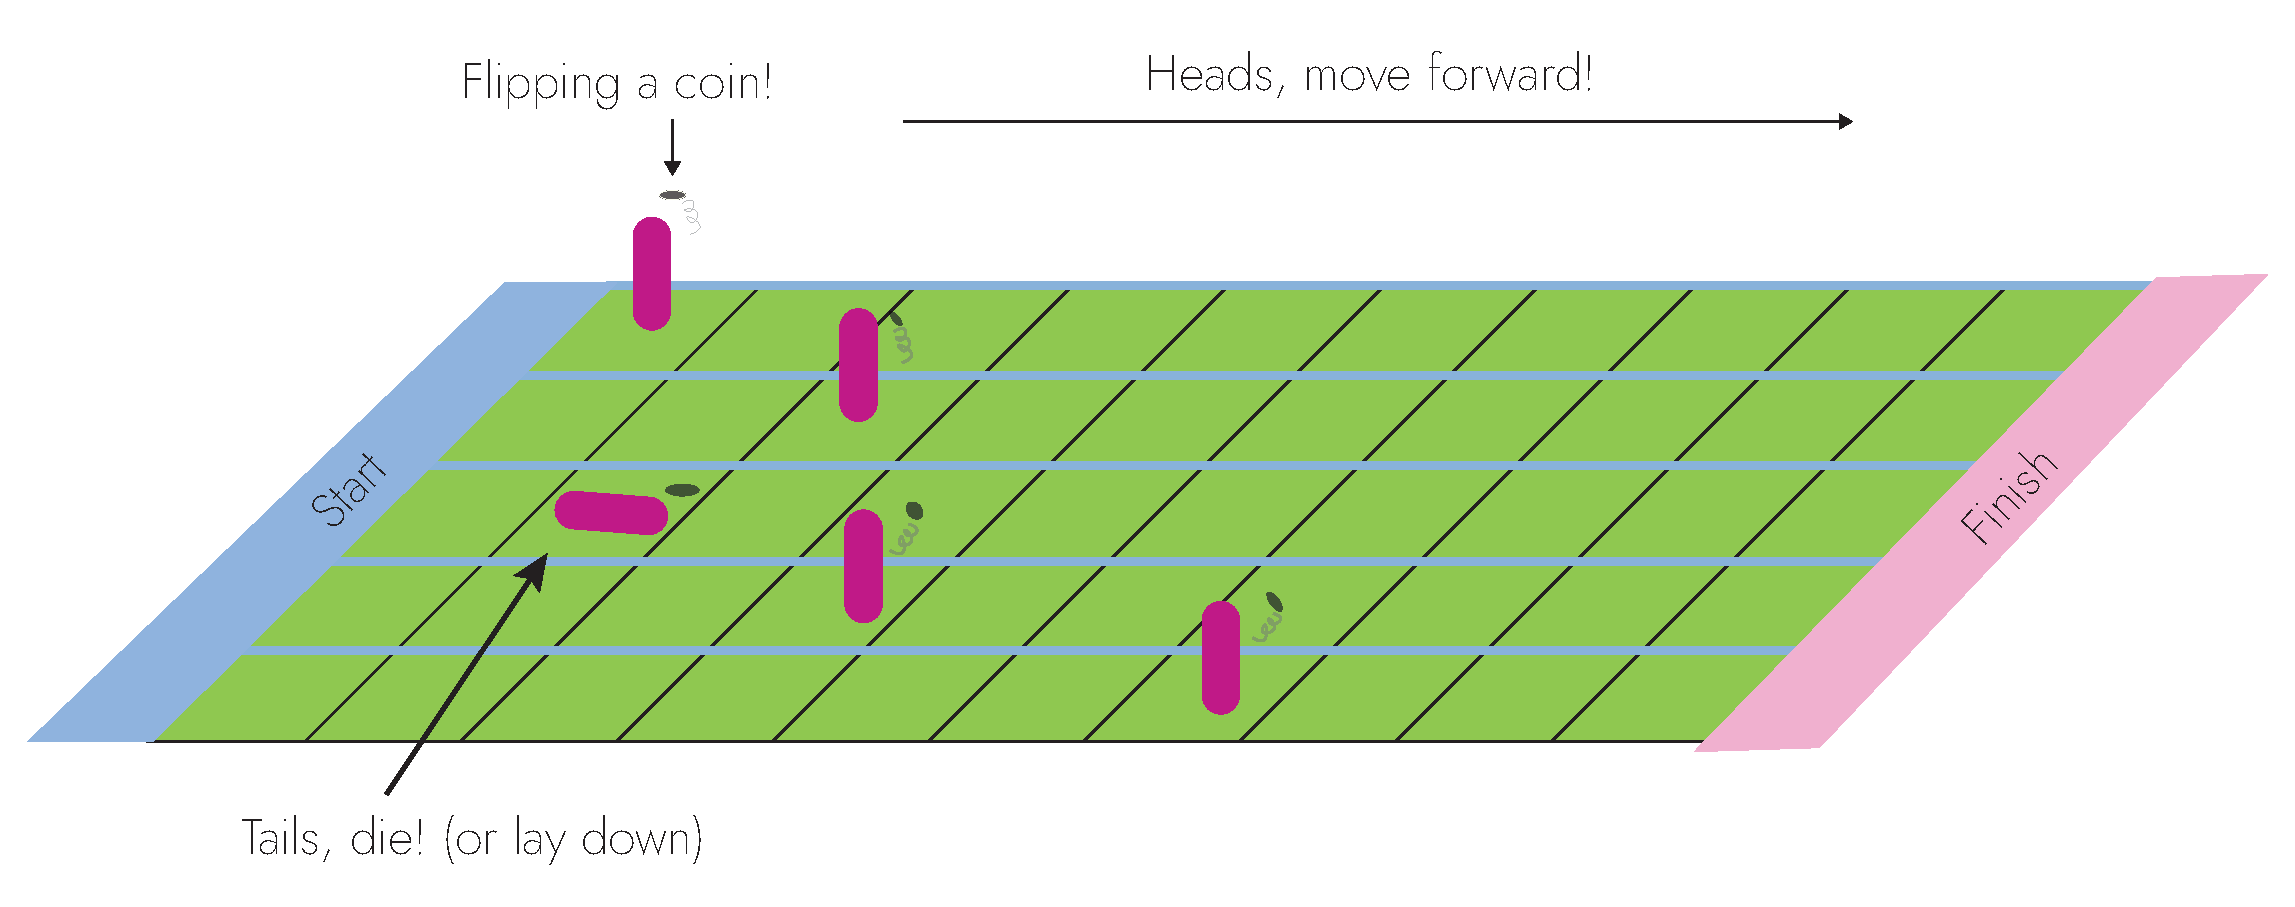
\includegraphics{coin_flipping_schematicpdf.jpg}

But let's make it more interesting! Let's assume that the coin can be
super biased. Instead of a 50\% chance of dying, I manipulate it so that
the chance of getting tails can vary from 1\% to 100\%. Also let's
assume that I introduce some variability. Some friends can only take a
small step and other friends can take larger steps. They somehow need to
cumulatively take 10 paces to win, but you can see that there are
advantages to those who can very large steps.

My question is what does it look like at the end of the finish line.
Specifically, what are the group of individuals that are able to finish
(do take small steps or big steps) and what is the timing? How does this
differ depending on what kind of coin I give them and what kind of steps
I allow them to take?

\subsection{The simplest code}\label{the-simplest-code}

For the death function, I'm going to use sample until I think a bit more
about the gritty mathematics. There is a binary outcome: you survived in
this timestep or you perished in this timestep. But we can directly
manipulate the probability of mortality.

\begin{Shaded}
\begin{Highlighting}[]
\NormalTok{death\_function }\OtherTok{\textless{}{-}} \ControlFlowTok{function}\NormalTok{(size, mort\_prob)\{}
\NormalTok{  sampled }\OtherTok{\textless{}{-}} \FunctionTok{sample}\NormalTok{(}\FunctionTok{c}\NormalTok{(}\DecValTok{0}\NormalTok{,}\DecValTok{1}\NormalTok{), size,}\AttributeTok{replace =} \ConstantTok{TRUE}\NormalTok{, }\AttributeTok{prob =}\FunctionTok{c}\NormalTok{(mort\_prob, }\DecValTok{1}\SpecialCharTok{{-}}\NormalTok{ mort\_prob))}
  \FunctionTok{return}\NormalTok{(sampled)}
\NormalTok{\}}
\end{Highlighting}
\end{Shaded}

Now, how do our friends progress through the lawn game. We can give
everyone a number (1,2,3) and depending on your number, you can take
large steps or very small. You can see that if you are in Group 1, you
take smaller steps than individuals in Group 3.

\begin{Shaded}
\begin{Highlighting}[]
\NormalTok{progress\_function }\OtherTok{\textless{}{-}} \ControlFlowTok{function}\NormalTok{(id)\{}
  
  \ControlFlowTok{if}\NormalTok{(id }\SpecialCharTok{==}\DecValTok{1}\NormalTok{)\{}
\NormalTok{  sampled }\OtherTok{\textless{}{-}} \FunctionTok{runif}\NormalTok{(}\DecValTok{1}\NormalTok{,}\AttributeTok{min =}\DecValTok{0}\NormalTok{, }\AttributeTok{max =}\DecValTok{3}\NormalTok{)}
\NormalTok{  \}}
  \ControlFlowTok{else} \ControlFlowTok{if}\NormalTok{ (id }\SpecialCharTok{==}\DecValTok{2}\NormalTok{)\{}
\NormalTok{  sampled }\OtherTok{\textless{}{-}} \FunctionTok{runif}\NormalTok{(}\DecValTok{1}\NormalTok{,}\AttributeTok{min =} \DecValTok{2}\NormalTok{,}\AttributeTok{max=}\DecValTok{5}\NormalTok{)}
\NormalTok{  \}}
  \ControlFlowTok{else} \ControlFlowTok{if}\NormalTok{ (id }\SpecialCharTok{==}\DecValTok{3}\NormalTok{)\{}
\NormalTok{  sampled }\OtherTok{\textless{}{-}} \FunctionTok{runif}\NormalTok{(}\DecValTok{1}\NormalTok{,}\AttributeTok{min =} \DecValTok{5}\NormalTok{, }\AttributeTok{max =}\DecValTok{10}\NormalTok{)}
\NormalTok{  \}}
  \FunctionTok{return}\NormalTok{(sampled)}
\NormalTok{\}}
\end{Highlighting}
\end{Shaded}

Now here is the most convoluted code of how the race can begin. A gist
of it is that for anyone who has not died, I make them flip the coin. If
it's 0, they stay in place and I record at what time they `died'. If
it's a 1, they are still alive where they can make progress to winning.
If they accumulate 10 steps, then they won and they wait while everyone
finishes (by either `dying' or `winning').

\begin{Shaded}
\begin{Highlighting}[]
\NormalTok{lawn\_race\_function }\OtherTok{\textless{}{-}} \ControlFlowTok{function}\NormalTok{(size, mort\_prob, progress\_time,time\_step) \{}
\NormalTok{  full\_df }\OtherTok{\textless{}{-}} \FunctionTok{data.frame}\NormalTok{(}
      \AttributeTok{current\_time =} \FunctionTok{rep}\NormalTok{(}\DecValTok{0}\NormalTok{, size),}
      \AttributeTok{time\_event =} \FunctionTok{rep}\NormalTok{(}\DecValTok{0}\NormalTok{, size),}
      \AttributeTok{status =} \FunctionTok{rep}\NormalTok{(}\DecValTok{1}\NormalTok{, size),}
      \AttributeTok{progress =} \FunctionTok{rep}\NormalTok{(}\DecValTok{0}\NormalTok{, size),}
       \AttributeTok{id =} \FunctionTok{rep}\NormalTok{(}\FunctionTok{c}\NormalTok{(}\DecValTok{1}\NormalTok{, }\DecValTok{2}\NormalTok{, }\DecValTok{3}\NormalTok{), }\AttributeTok{length =}\NormalTok{ size),}
       \AttributeTok{friend\_number =} \FunctionTok{seq}\NormalTok{(}\DecValTok{1}\NormalTok{, size))}

\NormalTok{  survived\_subsetted }\OtherTok{\textless{}{-}}\NormalTok{ full\_df [full\_df }\SpecialCharTok{$}\NormalTok{status }\SpecialCharTok{==} \DecValTok{1}\NormalTok{ ,]}
  
\NormalTok{  i }\OtherTok{=} \DecValTok{0}
  
  \ControlFlowTok{while}\NormalTok{ (}\FunctionTok{nrow}\NormalTok{(full\_df [full\_df }\SpecialCharTok{$}\NormalTok{status }\SpecialCharTok{==} \DecValTok{1}\NormalTok{ ,]) }\SpecialCharTok{!=} \DecValTok{0}\NormalTok{) \{}
    
\NormalTok{    i }\OtherTok{=}\NormalTok{ i }\SpecialCharTok{+} \DecValTok{1}
\NormalTok{    dead\_developed\_already\_subsetted }\OtherTok{\textless{}{-}}\NormalTok{ full\_df[full\_df}\SpecialCharTok{$}\NormalTok{status }\SpecialCharTok{\%in\%} \FunctionTok{c}\NormalTok{(}\DecValTok{0}\NormalTok{,}\DecValTok{2}\NormalTok{),]}
\NormalTok{    survived\_subsetted }\OtherTok{\textless{}{-}}\NormalTok{ full\_df [full\_df }\SpecialCharTok{$}\NormalTok{status }\SpecialCharTok{==} \DecValTok{1}\NormalTok{ ,]}
\NormalTok{    survived\_individuals }\OtherTok{\textless{}{-}} \FunctionTok{nrow}\NormalTok{(survived\_subsetted)}
 \DocumentationTok{\#\#\#If there are surviving individuals}
      
\NormalTok{      survived\_subsetted}\SpecialCharTok{$}\NormalTok{current\_time }\OtherTok{\textless{}{-}}\NormalTok{ i}

      \DocumentationTok{\#\#\# Did they die in this time{-}step?}
\NormalTok{      survived\_subsetted}\SpecialCharTok{$}\NormalTok{status }\OtherTok{\textless{}{-}} \FunctionTok{death\_function}\NormalTok{(survived\_individuals, mort\_prob)}
      
      \ControlFlowTok{if}\NormalTok{(}\FunctionTok{nrow}\NormalTok{(  survived\_subsetted[survived\_subsetted}\SpecialCharTok{$}\NormalTok{status }\SpecialCharTok{==} \DecValTok{0}\NormalTok{, ])}\SpecialCharTok{!=}\DecValTok{0}\NormalTok{)\{}
      
\NormalTok{      survived\_subsetted[survived\_subsetted}\SpecialCharTok{$}\NormalTok{status }\SpecialCharTok{==} \DecValTok{0}\NormalTok{, ]}\SpecialCharTok{$}\NormalTok{time\_event }\OtherTok{\textless{}{-}}\NormalTok{ i}

\NormalTok{      \}}
      \DocumentationTok{\#\#\# Progressed}
\NormalTok{      growing\_indviduals }\OtherTok{\textless{}{-}}\NormalTok{ survived\_subsetted[survived\_subsetted}\SpecialCharTok{$}\NormalTok{status }\SpecialCharTok{==} \DecValTok{1}\NormalTok{, ]}

      \DocumentationTok{\#\#\#If there are those that will grow}
      \ControlFlowTok{if}\NormalTok{(}\FunctionTok{nrow}\NormalTok{(growing\_indviduals) }\SpecialCharTok{!=}\DecValTok{0}\NormalTok{)\{}
      
\NormalTok{      growing\_indviduals}\SpecialCharTok{$}\NormalTok{progress }\OtherTok{\textless{}{-}} \FunctionTok{round}\NormalTok{(growing\_indviduals }\SpecialCharTok{$}\NormalTok{progress }\SpecialCharTok{+} 
\NormalTok{                                            time\_step}\SpecialCharTok{*}\FunctionTok{sapply}\NormalTok{(}\AttributeTok{X =}\NormalTok{ growing\_indviduals }\SpecialCharTok{$}\NormalTok{id, }\AttributeTok{FUN =}\NormalTok{ progress\_function ), }\DecValTok{3}\NormalTok{)}

\NormalTok{      developed }\OtherTok{\textless{}{-}}\NormalTok{ growing\_indviduals[growing\_indviduals}\SpecialCharTok{$}\NormalTok{progress }\SpecialCharTok{\textgreater{}=}\NormalTok{ progress\_time, ]}

      \DocumentationTok{\#\#\#If there are those developed }
      \ControlFlowTok{if}\NormalTok{(}\FunctionTok{nrow}\NormalTok{(developed) }\SpecialCharTok{!=} \DecValTok{0}\NormalTok{)\{}
\NormalTok{      growing\_indviduals[growing\_indviduals}\SpecialCharTok{$}\NormalTok{progress }\SpecialCharTok{\textgreater{}=}\NormalTok{ progress\_time, ]}\SpecialCharTok{$}\NormalTok{status }\OtherTok{\textless{}{-}} \DecValTok{2}
\NormalTok{      growing\_indviduals[growing\_indviduals}\SpecialCharTok{$}\NormalTok{status }\SpecialCharTok{==} \DecValTok{2}\NormalTok{, ]}\SpecialCharTok{$}\NormalTok{time\_event }\OtherTok{\textless{}{-}}\NormalTok{ i}
\NormalTok{      \}}
\NormalTok{      \}}
      
\NormalTok{      full\_df }\OtherTok{\textless{}{-}} \FunctionTok{rbind}\NormalTok{(dead\_developed\_already\_subsetted ,}
\NormalTok{        survived\_subsetted[survived\_subsetted}\SpecialCharTok{$}\NormalTok{status }\SpecialCharTok{==} \DecValTok{0}\NormalTok{, ],}
\NormalTok{       growing\_indviduals}
\NormalTok{      )}
  
  
\NormalTok{  \}}
  \FunctionTok{return}\NormalTok{(full\_df)}
\NormalTok{\}}
\end{Highlighting}
\end{Shaded}

\subsection{The result}\label{the-result}

So I set two matches with 100,000 of my friends. The first match, the
probability of dying at each time step is 0.001 and you must make 10
steps to win. The second match, the probability of dying at each time
step is 0.10 and still you must take 10 steps to win. What does it look
like between the two races?

\begin{Shaded}
\begin{Highlighting}[]
\NormalTok{df\_lawn\_race1}\OtherTok{\textless{}{-}} \FunctionTok{lawn\_race\_function}\NormalTok{(}\FloatTok{1e5}\NormalTok{,}\FloatTok{0.01}\NormalTok{,}\DecValTok{10}\NormalTok{,}\AttributeTok{time\_step =} \DecValTok{1}\SpecialCharTok{/}\DecValTok{5}\NormalTok{)}
\NormalTok{df\_lawn\_race2}\OtherTok{\textless{}{-}} \FunctionTok{lawn\_race\_function}\NormalTok{(}\FloatTok{1e5}\NormalTok{,}\FloatTok{0.40}\NormalTok{,}\DecValTok{10}\NormalTok{,}\AttributeTok{time\_step =} \DecValTok{1}\SpecialCharTok{/}\DecValTok{5}\NormalTok{)}
\end{Highlighting}
\end{Shaded}

\begin{Shaded}
\begin{Highlighting}[]
\NormalTok{first\_panel }\SpecialCharTok{/}\NormalTok{ second\_panel }\SpecialCharTok{+}   \FunctionTok{plot\_layout}\NormalTok{(}\AttributeTok{guides =} \StringTok{\textquotesingle{}collect\textquotesingle{}}\NormalTok{)}
\end{Highlighting}
\end{Shaded}

\includegraphics{coin_flip_files/figure-latex/unnamed-chunk-8-1.pdf}

So it may be intuitive, but I like having this simulation and figure.
When you're in a race where the chance of mortality is very small, all
groups are able to effectively `win'. The slower group (Group 3 with the
star symbol!) may take a lot longer but eventually they will reach the
finish line. However, in the second situation (the bottom graph), with
greater chance for mortality, the one who are able to finish the race
faster (Group 1) are more likely to win. With each time step.

Let's take a new perspective

So everyone who won in the game, what does it look as a cumulative
proportion over time. The first race (dark green) and second race (blue)
are quite different!

\begin{verbatim}
## Warning: Using `size` aesthetic for lines was deprecated in ggplot2 3.4.0.
## i Please use `linewidth` instead.
## This warning is displayed once every 8 hours.
## Call `lifecycle::last_lifecycle_warnings()` to see where this warning was
## generated.
\end{verbatim}

\includegraphics{coin_flip_files/figure-latex/unnamed-chunk-11-1.pdf}

\begin{Shaded}
\begin{Highlighting}[]
\FunctionTok{ggplot}\NormalTok{(df\_full, }\FunctionTok{aes}\NormalTok{(}\AttributeTok{x =}\NormalTok{ time\_event, }\AttributeTok{y=}\NormalTok{ prop, }\AttributeTok{color =} \FunctionTok{as.factor}\NormalTok{(facet), }\AttributeTok{group =} \FunctionTok{as.factor}\NormalTok{(facet)))}\SpecialCharTok{+}
 \FunctionTok{geom\_line}\NormalTok{(}\AttributeTok{size =}\FloatTok{1.2}\NormalTok{)}\SpecialCharTok{+}
  \FunctionTok{xlab}\NormalTok{(}\StringTok{"Time"}\NormalTok{)}\SpecialCharTok{+}
  \FunctionTok{ylab}\NormalTok{(}\StringTok{"Cumulative proportion winning"}\NormalTok{)}\SpecialCharTok{+}
  \FunctionTok{scale\_color\_manual}\NormalTok{(}\AttributeTok{name =} \StringTok{"Race"}\NormalTok{,}\AttributeTok{values =} \FunctionTok{c}\NormalTok{(}\StringTok{\textasciigrave{}}\AttributeTok{1}\StringTok{\textasciigrave{}} \OtherTok{=} \StringTok{\textquotesingle{}darkgreen\textquotesingle{}}\NormalTok{, }\StringTok{\textasciigrave{}}\AttributeTok{2}\StringTok{\textasciigrave{}} \OtherTok{=} \StringTok{\textquotesingle{}blue\textquotesingle{}}\NormalTok{))}\SpecialCharTok{+}
  \FunctionTok{theme\_classic}\NormalTok{()}\SpecialCharTok{+}
 \FunctionTok{theme}\NormalTok{(}\AttributeTok{axis.text =} \FunctionTok{element\_text}\NormalTok{(}\AttributeTok{size =} \DecValTok{14}\NormalTok{),}
        \AttributeTok{axis.title =} \FunctionTok{element\_text}\NormalTok{(}\AttributeTok{size =} \DecValTok{14}\NormalTok{))}\SpecialCharTok{+}\FunctionTok{xlim}\NormalTok{(}\DecValTok{0}\NormalTok{,}\DecValTok{60}\NormalTok{)}
\end{Highlighting}
\end{Shaded}

\includegraphics{coin_flip_files/figure-latex/unnamed-chunk-12-1.pdf}

Huh\ldots{} Could there be more variability of individuals winning in
the first race?

\end{document}
